\documentclass[border=6pt]{standalone}
\usepackage{tikz}
\usetikzlibrary{arrows.meta,positioning,calc}
\begin{document}
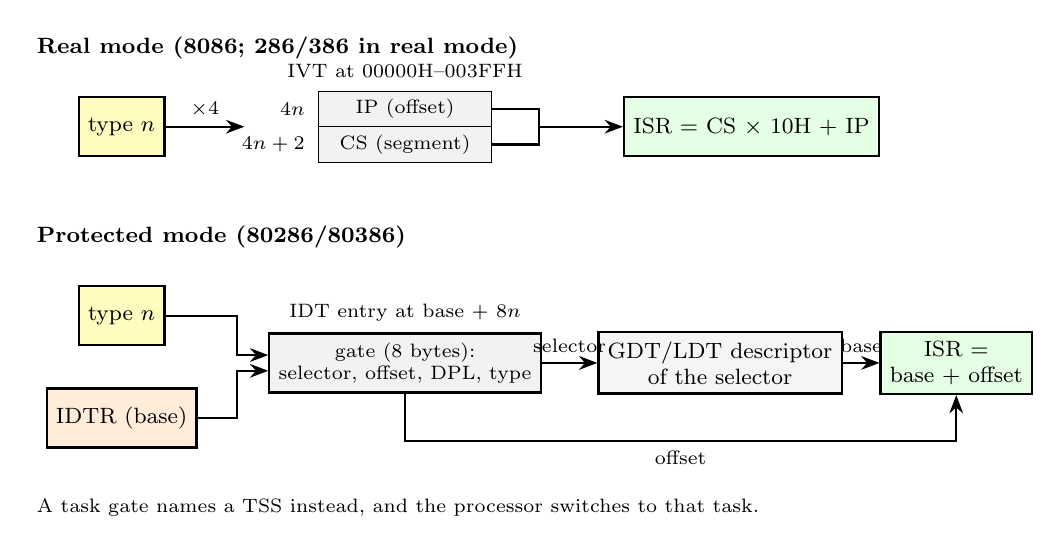
\begin{tikzpicture}[>=Stealth,font=\small,
 b/.style={draw,thick,align=center,font=\footnotesize,minimum height=0.75cm},
 cell/.style={draw,minimum width=2.2cm,minimum height=0.45cm,font=\scriptsize,inner sep=0}]
% real mode
\node[font=\footnotesize\bfseries,anchor=west] at (-1.2,1.0) {Real mode (8086; 286/386 in real mode)};
\node[b,fill=yellow!25] (n) at (0,0) {type $n$};
\node[cell,fill=gray!10] (ip) at (3.6,0.225) {IP (offset)};
\node[cell,fill=gray!10] (cs) at (3.6,-0.225) {CS (segment)};
\node[font=\scriptsize,anchor=east] at (2.45,0.225) {$4n$};
\node[font=\scriptsize,anchor=east] at (2.45,-0.225) {$4n+2$};
\node[font=\scriptsize,anchor=south] at (3.6,0.5) {IVT at 00000H--003FFH};
\draw[->,thick] (n.east) -- ++(1.0,0) node[pos=0.5,above,font=\scriptsize]{$\times 4$};
\node[b,fill=green!10] (isr1) at (8.0,0) {ISR = CS $\times$ 10H + IP};
\draw[thick] (ip.east) -- (5.3,0.225) -- (5.3,-0.225) -- (cs.east);
\draw[->,thick] (5.3,0) -- (isr1.west);
% protected mode
\begin{scope}[yshift=-2.4cm]
\node[font=\footnotesize\bfseries,anchor=west] at (-1.2,1.0) {Protected mode (80286/80386)};
\node[b,fill=yellow!25] (n2) at (0,0) {type $n$};
\node[b,fill=orange!15] (idtr) at (0,-1.3) {IDTR (base)};
\node[draw,thick,fill=gray!10,minimum width=2.6cm,minimum height=0.75cm,font=\scriptsize,align=center] (gate) at (3.6,-0.6) {gate (8 bytes):\\selector, offset, DPL, type};
\node[font=\scriptsize,anchor=south] at (3.6,-0.2) {IDT entry at base + $8n$};
\draw[->,thick] (n2.east) -| ($(gate.west)+(-0.4,0.1)$) -- ($(gate.west)+(0,0.1)$);
\draw[->,thick] (idtr.east) -| ($(gate.west)+(-0.4,-0.1)$) -- ($(gate.west)+(0,-0.1)$);
\node[b,fill=gray!8] (desc) at (7.6,-0.6) {GDT/LDT descriptor\\of the selector};
\draw[->,thick] (gate.east) -- (desc.west) node[midway,above,font=\scriptsize]{selector};
\node[b,fill=green!10] (isr2) at (10.6,-0.6) {ISR =\\base + offset};
\draw[->,thick] (desc.east) -- (isr2.west) node[midway,above,font=\scriptsize]{base};
\draw[->,thick] (gate.south) -- ++(0,-0.6) -| (isr2.south) node[pos=0.25,below,font=\scriptsize]{offset};
\node[font=\scriptsize,anchor=north west] at (-1.2,-2.2) {A task gate names a TSS instead, and the processor switches to that task.};
\end{scope}
\end{tikzpicture}
\end{document}
